\section{Introduction}

We build a library to help inter-operability between codes
in the field of quantum chemistry, primarily focussed on enabling the
communication of data between the flagship codes of the \ac{TREX}
\ac{CoE} (NECI, GammCor, Quantum Package, QMC=Chem, CHAMP, TurboRVB,
QML). We expect this library to be also adopted by the community beyond
\ac{TREX}.
The data which needs to be stored is the electronic wave function
obtained from a post-Hartree-Fock calculation, or the one- and
two-body density matrices together with the one- and two- electron
integrals necessary to compute the energy or other properties.
As a wave function can be obtained by executing multiple codes
in a complex workflow, the library should give the possibility to
build the files incrementally using multiple codes.

\begin{figure}[h]
  \centering
  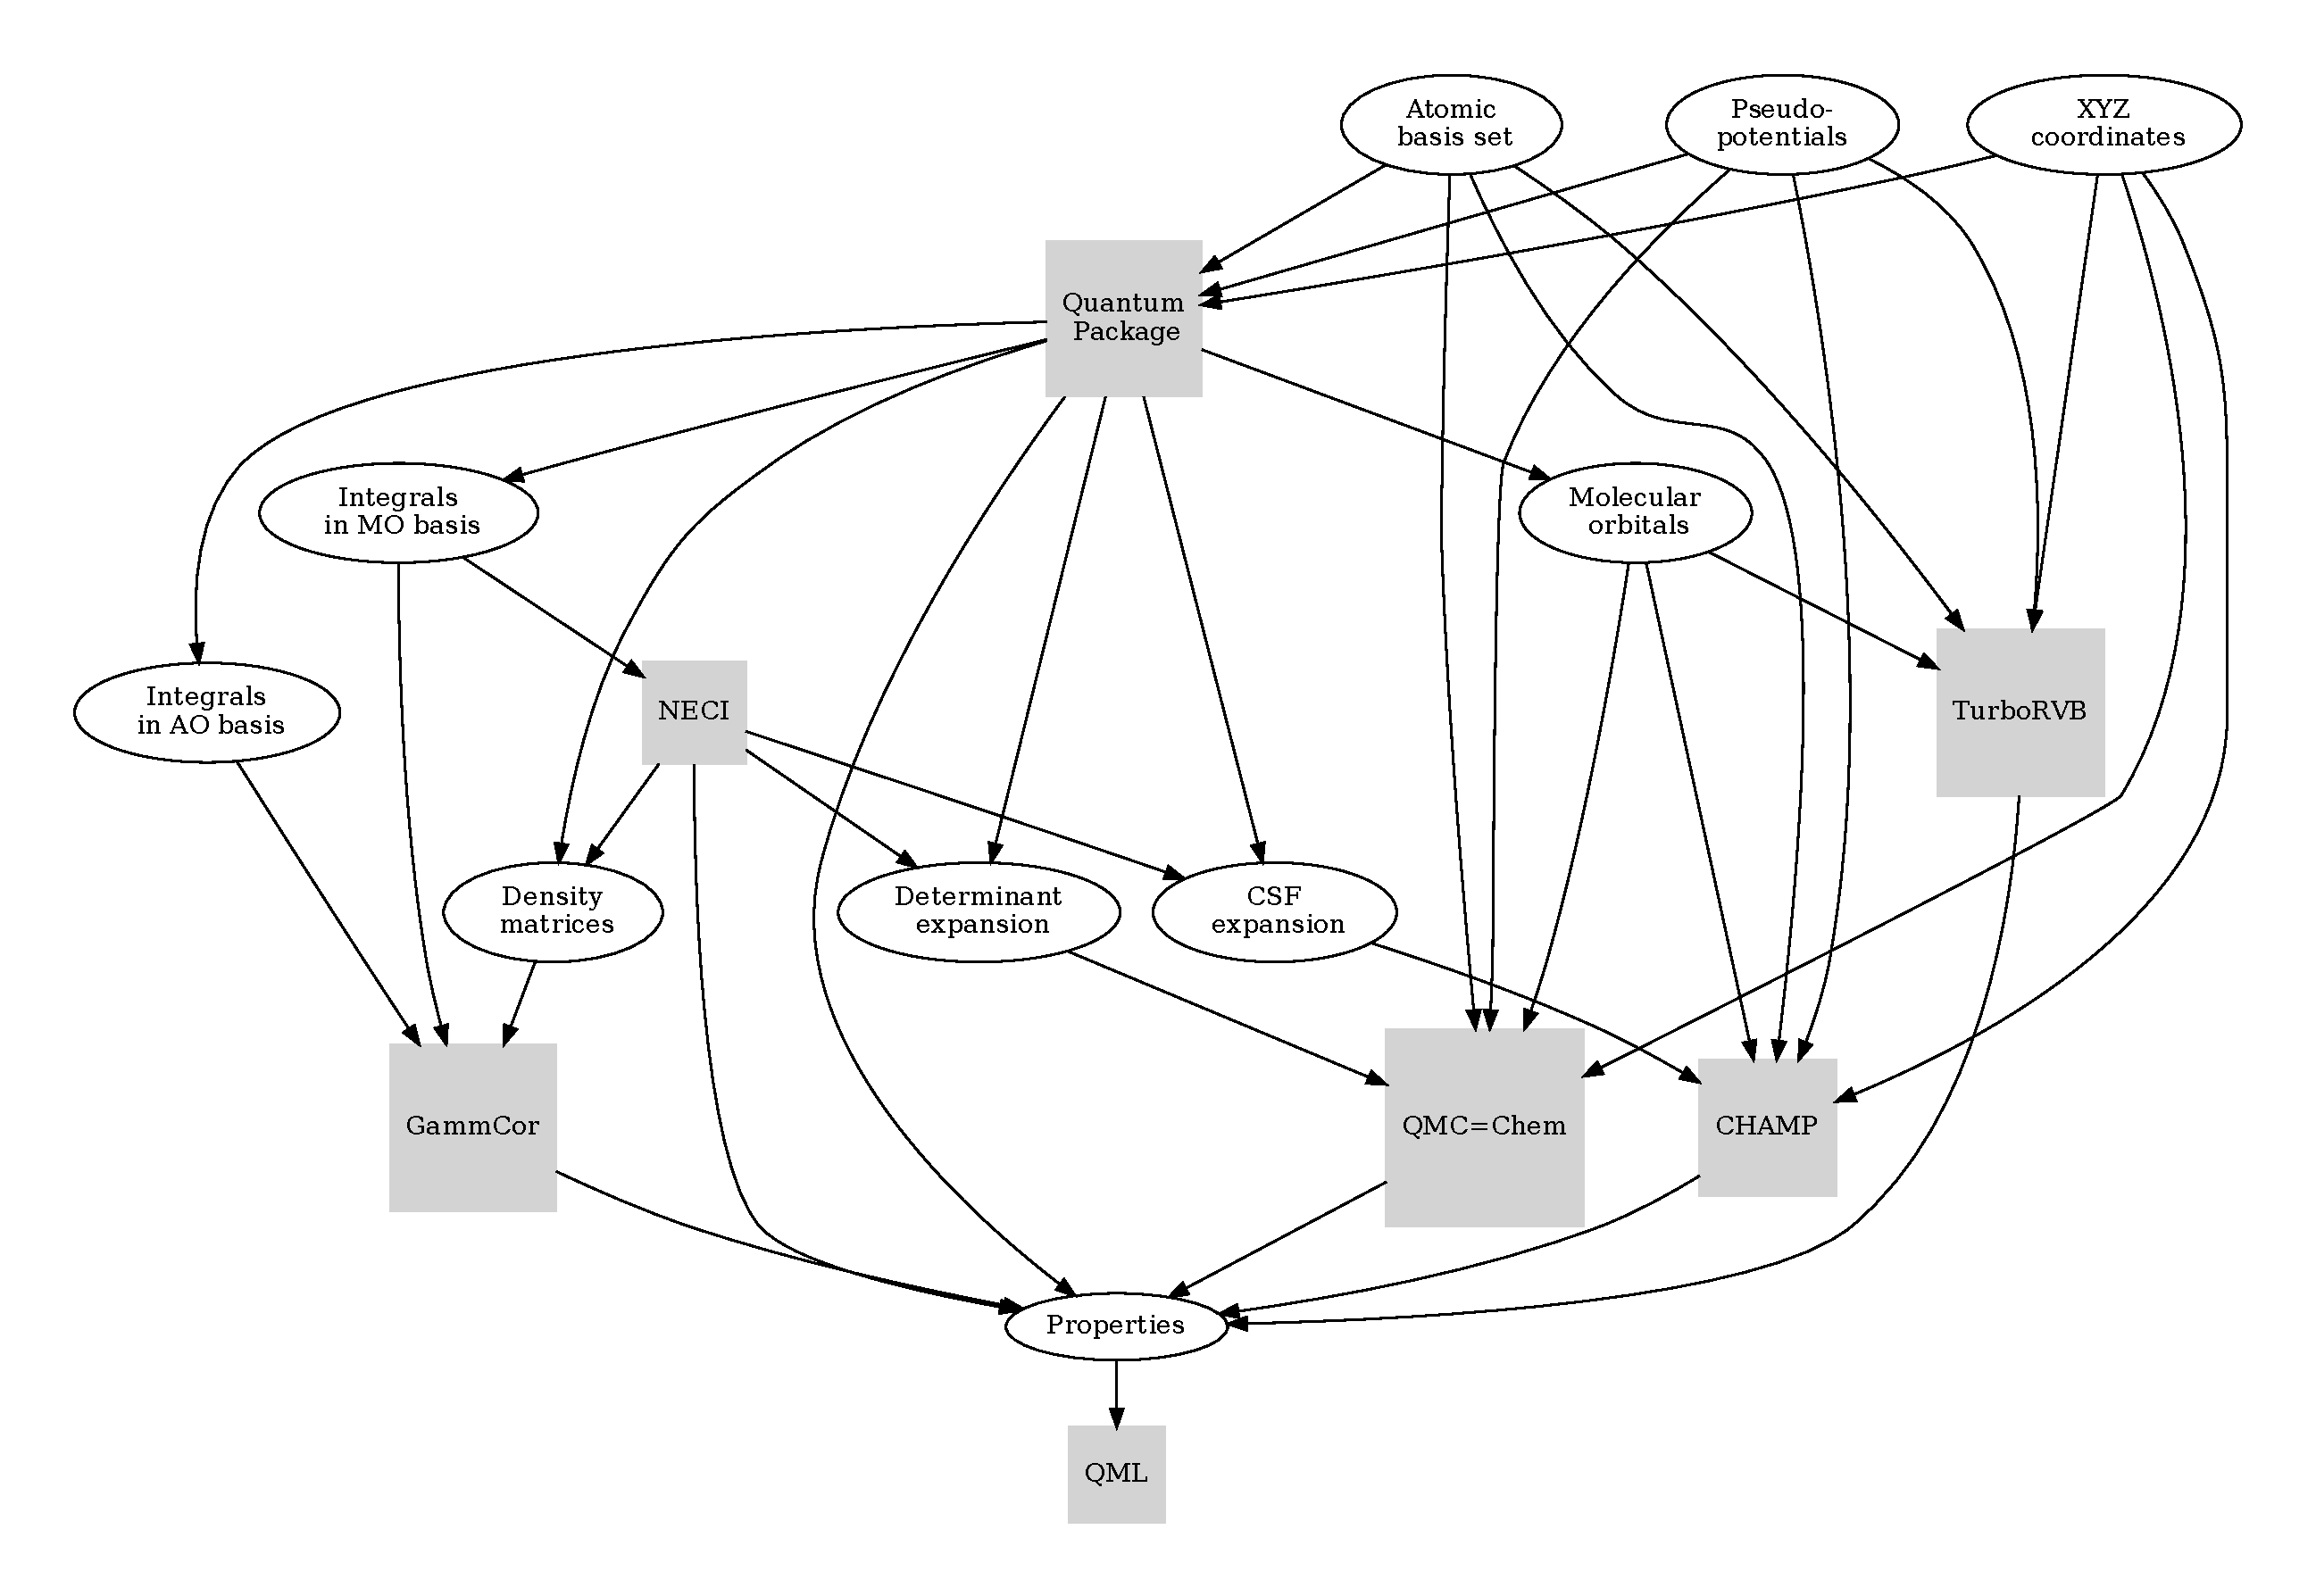
\includegraphics[width=\textwidth]{codes.pdf}
  \caption{Dependencies between the codes and the data. Codes are
    represented in grey, and data are represented in white.}
  \label{fig:codes}
\end{figure}

Fig.~\ref{fig:codes} shows which data is read and written by all of
the codes of the \ac{TREX} \ac{CoE}. The objective of this library is
to organize all the data in a file, and provide a common interface to
make the data accessible easily to all the codes.

\section{Content of the files}

The files need to be self-contained: they should contain
\emph{all} the information needed to reconstruct the wave functions
from an external program, without relying on any extra service to
provide additional data.
For instance, all the parameters of the atomic basis set should be
explicitly stored instead of storing only the conventional name of the
basis, which would require obtaining the parameters from another
source. Being self-contained is important if the files are archived
on an open-data repository: it reduces the dependencies to other
services and therefore increases re-usability.

\subsection{Metadata}

As we expect our files to be archived in open-data repositories, we
need to give the possibility to the users to store some metadata
inside the files.

\subsection{Nuclei}

We consider wave functions where the nuclei are considered as fixed
point charges. The file should contain information decribing the
positions of the nuclei, their charges, their labels, and the
point-group symmetry of the system.

\subsection{Electrons}

We consider wave functions expressed in the spin-free formalism, where
the number of $\uparrow$ and $\downarrow$ electrons is
fixed. Therefore, specifying the numbers of $\uparrow$ and
$\downarrow$ suffices to determine the spin multiplicity and the
magnetic quantum number.

\subsection{Atomic Basis set}

We consider here basis functions centered on nuclei. Hence, we enable
the possibility to define \emph{dummy atoms} to place basis functions
in random positions.

The atomic basis set is defined as a list of shells. Each shell $s$ is
centered on a nucleus $A$, possesses a given angular momentum $l$ and a
radial function $R_s$. The radial function is a linear combination of
\emph{primitive} functions that can be of type Slater ($p=1$)  or
Gaussian ($p=2$):
\[
  R_s(\mathbf{r}) = \mathcal{N}_s |\mathbf{r}-\mathbf{R}_A|^{n_s}
  \sum_{k=1}^{N_{\text{prim}}} a_{ks}
 \exp \left( - \gamma_{ks} 
  |\mathbf{r}-\mathbf{R}_A|^p \right).
\]
In the case of Gaussian functions, $n_s$ is always zero.
The normalization factor $\mathcal{N}_s$ ensures that all the functions
of the shell are normalized to unity. As this normalization requires
the ability to compute overlap integrals, it should be written in the
file to ensure that the file is self-contained and does not require
the client program to have the ability to compute such integrals.

\subsection{Atomic Orbitals}

Going from the atomic basis set to \acp{AO} implies a systematic
construction of all the angular functions of each shell.
We consider two cases for the angular functions: the real spherical
harmonics, and the polynomials in cartesian coordinates.
In the case of spherical harmonics, the \acp{AO} are ordered in
increasing magnetic quantum number ($-l \le m \le l$), and in the case
of polynomials we choose the canonical ordering of the
\texttt{Libint}\cite{Libint2} library, i.e
\begin{eqnarray}
p & : & p_x, p_y, p_z \nonumber \\
d & : & d_{xx}, d_{xy}, d_{xz}, d_{yy}, d_{yz}, d_{zz} \nonumber \\
f & : & f_{xxx}, f_{xxy}, f_{xxz}, f_{xyy}, f_{xyz}, f_{xzz}, f_{yyy}, f_{yyz}, f_{yzz}, f_{zzz} \nonumber \\
{\rm etc.} \nonumber
\end{eqnarray}

\acp{AO} are defined as
\[
  \chi_i (\mathbf{r}) = P_{\eta(i)}(\mathbf{r})\, R_{\theta(i)} (\mathbf{r})
\]
where $\theta(i)$ returns the shell on which the \ac{AO} is expanded,
and $\eta(i)$ denotes which polynomial is chosen.

\subsection{Effective core potentials}
It is common practice to use \ac{ECP} in \ac{QMC} calculations.  An
\ac{ECP} $V_A^{\text{pp}}$ replacing the core electrons of atom $A$ is
the sum of a local component $V_A^{\text{loc}}$ and a non-local
component $V_A^{\text{non-loc}}$.\cite{burkatzki_2008}
The local component is given by
\[
  V_A^{\text{loc}}(r) = -\frac{Z_A^{\text{eff}}}{r} +
  \frac{Z_A^{\text{eff}}}{r}\, \exp\left( -\alpha_A\, r^2\right) + 
  Z_{\text{eff}}\, \alpha_A\, r\, \exp\left( -\beta_A\, r^2\right) + 
  \gamma_A \exp\left( -\delta_A\, r^2\right),
\]
and the non-local component is
\[
  V_A^{\text{non-loc}}(r) =
    \zeta_A\, \exp\left( -\eta_A\, r^2\right) |0\rangle \langle 0| +  
    \mu_A \,  \exp\left( -\nu_A \, r^2\right) |1\rangle \langle 1|
\]
where $r=|\mathbf{r-R}_A|$ is the distance to the nucleus on which the
potential is centered.


\subsection{One-electron integrals in the AO basis set}

The one-electron integrals of the form
\[
  O_{ij} = \int \chi_i(\mathbf{r})\, \hat{O}\, \chi_j(\mathbf{r}) \text{d}\mathbf{r},
\]
where $\hat{O}$ is a one-electron operator. The integrals needed to
compute the energy are the overlap integrals $\mathbf{S}$ with $\hat{O}=\mathbf{1}$,
the kinetic energy integrals $\mathbf{T}$ with $\hat{O}=\mathbf{\nabla}$, the
electron-nucleus potential integrals $\mathbf{V}$ with $\hat{O}=-\sum_A
Z_A^{\text{eff}}/|\mathbf{r-R}_A|$,
and the effective core potential integrals $\mathbf{V}^{\text{pp}}$
with $\hat{O}=V^{\text{pp}}$.

It is also convenient to store the \emph{core Hamiltonian} integrals, defined as
the sum of all the previously mentioned one-electron integrals.

\subsection{Two-electron integrals in the AO basis set}
\subsection{One-electron integrals in the MO basis set}
\subsection{Two-electron integrals in the MO basis set}


\subsection{Summary}

Table~\ref{tab:data}, summarizes the data that need to be stored in
the files.
\begin{longtable}{|l|l|}
  \caption{Information which should be stored in the file.\label{tab:data}}
  \\
\hline
Metadata
& File description    \\
& Code used to write the file \\
& Authors of the file         \\
\hline
Nuclei 
& Number of nuclei \\
& Atomic charges  \\
& XYZ coordinates \\
& Atom labels \\
& Point-group Symmetry \\
\hline
Electrons
& Number of $\uparrow$ and $\downarrow$ electrons \\
\hline
\ac{ECP}
  & Effective charge \\
  & Exponents of the local component \\
  & Coefficients of the local component \\
  & Powers of $r$ in the of the local component \\
  & Exponents of the non-local component \\
  & Coefficients of the non-local component \\
  & Powers of $r$ in the of the non-local component \\
\hline
Atomic basis set
  & Type : Gaussian or Slater \\
  & Cartesian or spherical coordinates \\
  & Normalization factors of the shells \\
  & Nuclei on which the functions are centered \\
  & Angular momenta \\
  & Exponents of the primitives \\
  & Coefficients of the primitives \\
\hline
  One-electron integrals in the AO basis 
 & Overlap integrals \\
 & Kinetic energy \\
 & Potential energy \\
 & Local component of the ECP \\
 & Non-Local component of the ECP \\
 & Core Hamiltonian \\
\hline
  Two-electron integrals in the AO basis 
 & Array of indices of \ac{ERI} \\
 & Array of values of \ac{ERI}  \\
 & Array of indices of long-range \ac{ERI} \\
 & Array of values of long-range \ac{ERI}  \\
\hline
Molecular orbitals
 & Type : Hartree-Fock, Localized, Natural, \dots \\
 & Coefficients \\
 & Class : Core, Inactive, Active, Virtual, Deleted, \dots \\
 & Symmetry \\
 & Occupation number \\
\hline
  One-electron integrals in the MO basis 
 & Kinetic energy \\
 & Potential energy \\
 & Local component of the ECP \\
 & Non-Local component of the ECP \\
 & Core Hamiltonian \\
\hline
  Two-electron integrals in the MO basis 
 & Array of indices of \ac{ERI} \\
 & Array of values of \ac{ERI}  \\
 & Array of indices of long-range \ac{ERI} \\
 & Array of values of long-range \ac{ERI}  \\
\hline
\end{longtable}



\section{Design of the library}

The design of the library is split in two disctinct sections: the
front end, and the back end. The front end is the interface between
the users and the library, and the back end is the interface between
the library and the physical storage. The library is designed to
decouple as much as possible the front end from the back end.

\subsection{License}

The library is licensed under the open-source 3-clause BSD license to facilitate
its adoption in all quantum chemistry software, commercial or not.

\subsection{The front end}


Most of the codes of the \ac{CoE} are written in Fortran, with some
scripts in Python. Therefore, the \ac{API} should be such that the
functions can be called easily in Fortran, and such that a Python
interface to the library is easy to write. These constraints have lead
us to the choice of implementing the library in C, with interfaces for
Fortran and Python.

To maximize the portability of the library, the stored data is reduced
to the subset of elementary C types: 32-/64-bit integers and floats,
scalar or arrays. The integer types defined in \mintinline{C}{<stdint.h>}
(\mintinline{C}{int64_t} and \mintinline{C}{int32_t}) are
used instead of the native C integer types.
Boolean variables are stored as integers, \mintinline{C}{1} for \mintinline{C}{true}
and \mintinline{C}{0} for \mintinline{C}{false}, and complex number are represented
as an array of two floats, the real part at address \mintinline{C}{0} and the
imaginary part at address \mintinline{C}{1}.

From table~\ref{tab:data}, it appears clearly that the data can be
organized in a tree structure, where the root of the tree is the file,
elementary pieces of data are leaves of the tree, and the nodes
between the root and the leaves constitute groups.

The \ac{API} is automatically generated from a configuration file
\texttt{trex.config}:
\inputminted[fontsize=\footnotesize]{fortran}{trex.config}



\subsection{The back end}

We want the data to be organized in the file, reproducing the
hierarchy of the data.

Using a binary format is desirable for the performance of large data
sets, such as integrals or density matrices, but binary files are not
necessarily compatible between different architectures because of the
endianness of the processors. Hence, if we store data in binary
format, the library should make the files machine-independent handling
the endianness of the binary representation.

Finally, as the produced files are likely to be archived on open data
repositories, it is desirable to have the possibility to compress them
efficiently.

The \ac{HDF5} file format and library\cite{hdf5} address properly these aspects:


HDF5 is large piece of software, which might not be installed on some
systems. If our library only provides an HDF5 back end, the users
unable to install HDF5 will not be able to use our library, and
therefore will not be able to use any of the \ac{TREX} code. Hence, we need
to protect our users for these situations.

We also provide a text-file back end. This back end is by far less
performant, but is has the advantage that it requires no dependencies.
We also provide a tool to convert files from the HDF5 format to the
text format, to ensure that if some large data has been prepared in
the HDF5 format, it can be converted to the text file format for
following calculations.




\subsection{Conventions}

We have defined some strong conventions to facilitate the
understanding of the users, and using as few exceptions as possible
makes it easier to guess the answers to their questions.
\begin{itemize}
  \item All the data are stored in atomic units.
  \item The singular is always used for the names of the variables.
  \item The \texttt{num} suffix denotes counting. For example
    \texttt{apple\_num} is the number of apples.
  \item All the variables that are used in array dimensions are 64-bit
    integers (\texttt{integer*8} in Fortran). This will avoid the
    integer overflows.
\end{itemize}

\section{Prototype library}

A prototype was created using following the design exposed in the
previous section, and is available in a repository under the \ac{TREX}
GitHub organization\footnote{\url{https://github.com/trex-coe/trex-io-prototype}}.

This prototype uses the \ac{EZFIO} library generator as a back end to
generate the stored files. This enabled us to focus on the front end,
which is the direct interface to the users.

